%%reuslts 
This chapter explains the results obtained after carrying out the Data Analysis process. It demonstrates key reuse across numerous hosts 
through the help of graph visualisations and other tables to provide an in-depth analysis of the clusters. This chapter also provides 
insights into the results obtained after optimisation and how it affected the program's run time and memory usage.

\section{Overview of Results}
\label{overview}
\begin{figure}[h!]
    \centering
    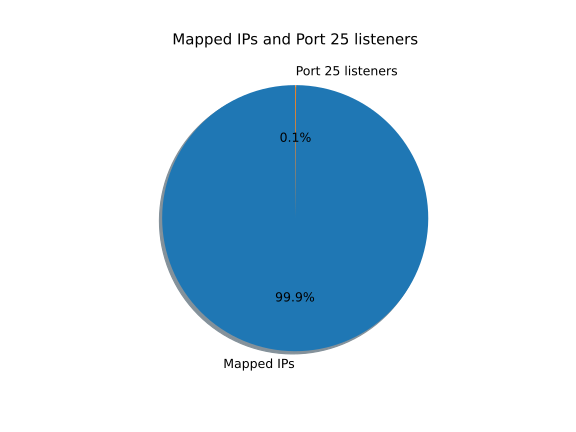
\includegraphics[width=13cm]{mapped-p25.png}
    \caption{IE Port 25 listeners}
    \label{fig:mappedp25}
\end{figure}
\pagebreak

\begin{figure}[h!]
    \centering
    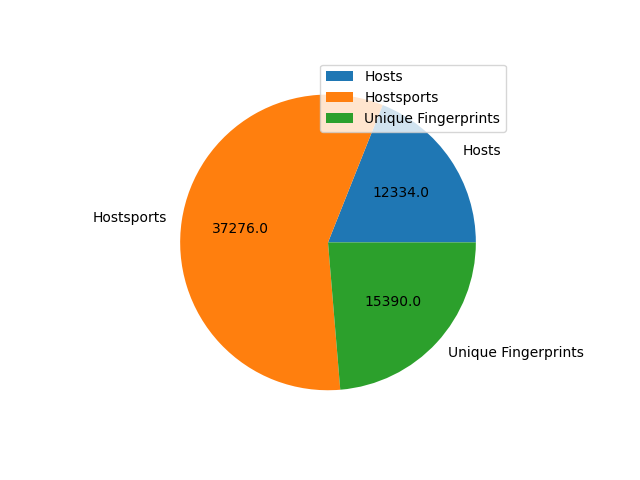
\includegraphics[width=14cm]{hostsports.png}
    \caption{Hosts v/s Host Ports v/s Fingerprints}
    \label{fig:hostports}
\end{figure}

\noindent Figure~\ref{fig:mappedp25} shows the number of IP addresses identified by ZMap as port 25 listeners. Out of the total IPs for Ireland (16421058), only 17,665 
were identified as mail servers making it 0.1\% of the total IPv4s assigned to Ireland.\\\\
12,333 hosts did some cryptography out of the 17,665 hosts identified as port 25 listeners, as indicated by figure~\ref*{fig:hostports}. 
Out of 12,333, about 37,276 host-ports combinations did some cryptography, but there were only 15,390 (41\%) unique fingerprints seen throughout the scans.
As only 41\% fingerprints were unique, it can be concluded that there is key sharing among hosts. The sections below further analyse this key 
reuse and provide analysis of some of the intriguing clusters found. 

\section{Protocol Versions}

\subsection{Cryptography per port Count}
\begin{figure}[h!]
    \centering
    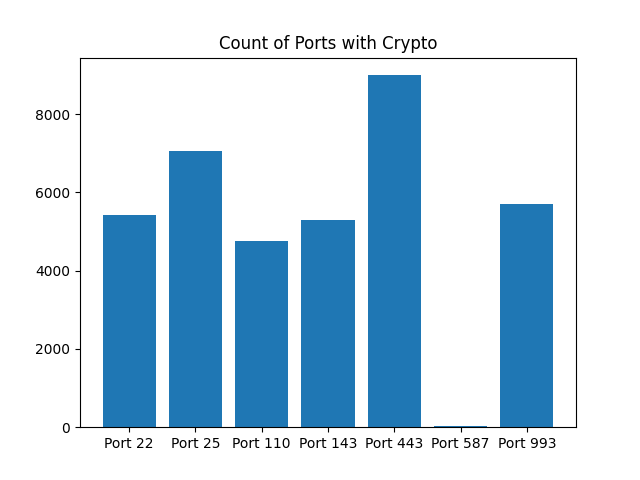
\includegraphics[width=12cm]{crypto-count.png}
    \caption{Ports that offer Crpto}
    \label{fig:cryptocount}
\end{figure}

\noindent Figure~\ref{fig:cryptocount} (below) depicts how many ports do some sort of cryptography across all IP addresses. Surprisingly, only 32 hosts on port 587 were found 
to be offering cryptographic services, and port 443 had the most number of hosts.
\subsection{SSH Versions}
\begin{figure}[h!]
    \centering
    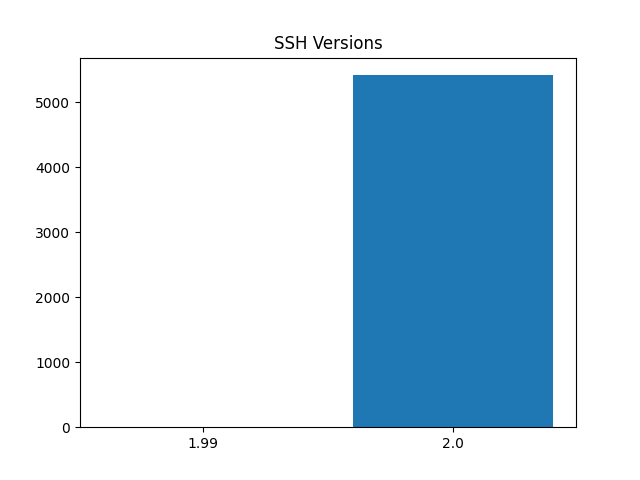
\includegraphics[width=10cm]{sshvers.png}
    \caption{SSH Versions}
    \label{fig:sshvers}
\end{figure}
\noindent Figure~\ref{fig:sshvers} above represents the SSH versions seen throughout the scans. Only two SSH versions are operating with only one host using them. 
SSH 1.9 and the rest of them using SSH 2.0. SSH 2.0 was introduced in 2006 and is the current standard version of SSH introduced by the IETF.
It provides significant improvements in terms of efficiency and security. SSH versions 1.0 and 2.0 are incompatible. Hence, SSH 1.9 was introduced by 
the IETF to provide some backward compatibility between the two versions~\cite{rfc4253}. 
\newpage

\subsection{TLS Versions}
\begin{table}[h!]
    \centering
    \begin{tabular}{|c|c|c|c|c|c|}
        \hline
        port  & SSLv3 & TLSv1.0 & TLSv1.1 & TLSv1.2 & Total  \\ \hline
        p25 & 0 & 120 & 4 & 6930 & 7054 \\ \hline
        p110 & 1 & 166 & 3 & 4600 & 4770 \\ \hline
        p143 & 0 & 179 & 3 & 5108 & 5290 \\ \hline
        p443 & 0 & 266 & 3 & 8729 & 8998 \\ \hline
        p587 & 0 & 2 & 0 & 30 & 32 \\ \hline
        p993 & 0 & 144 & 7 & 5563 & 5714 \\ \hline
        Total  & 1 & 877 & 20 & 30960 & 31858 \\ \hline
    \end{tabular}
    \caption{TLS Versions}
    \label{table:tlsvers}
\end{table}

\noindent Table~\ref*{table:tlsvers} shows the TLS versions seen throughout the scans irrespective of the IP address belonging to a cluster. Most of the TLS versions 
seen are TLS 1.2, followed by TLS 1.0, with the least SSLv3. There was no instance of TLS 1.3 in our scans. Surprisingly, it was observed 
that a significant number of hosts are still operating TLS 1.0, and some are employing TLS 1.1 even though both TLS versions have been depreciated by the 
IETF. The old versions were depreciated because of significant security flaws associated with the old versions. Some of the reasons behind 
the depreciation of TLS 1.0 and 1.1 are:
\begin{itemize}
    \item Old TLS versions require implementation using old cipher suites that are no longer desirable from a security point of view.
    \item Old versions do not support the modern and recommended cipher suites.
    \item The integrity of the handshake and the authentication process depend on SHA-1 hashes and signatures, respectively, which can easily be broken and has been superseded by SHA-2. 
\end{itemize} 
\noindent TLS 1.0 was released in 1999 and is considered to be the weakest of all TLS versions, and the IETF does explicitly not permit the use of it \cite{rfc8996}. 
This is because it is known to suffer from attacks like the BEAST due to improper implementation of the Cipher Block Chaining~\cite{rfc7457}.\\\\
Even though TLS 1.2 has also been upgraded by TLS 1.3, it was not seen during the scans. 
This might be because the TLS 1.3 upgrade is one of the most significant upgrades as compared to other TLS versions. The new upgrade introduced 
new features like 0-RTT that provide significant speed upgrades during a TLS connection establishment. Since TLS 1.3 was drastically different,
and due to middleboxes all over the internet, the TLS handshake might seem like a TLS 1.2 connection even though it is TLS 1.3~\cite{rfc8446}. 

\section{Key Reuse Results}
Five thousand eight hundred nine collisions were found, producing about 1049 clusters. The graphs below are a few of the selected clusters from 
the results. Some were selected based on the number of hosts, while others were chosen randomly.

\subsection{Cluster 15}
\begin{figure}[h!]
    \centering
    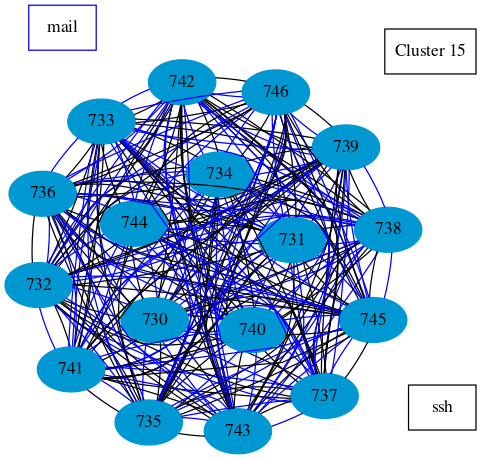
\includegraphics[width=10cm]{graph15.dot.png}
    \caption{Cluster 15}
    \label{fig:cluster15}
\end{figure}
\noindent Figure~\ref*{fig:cluster15} is the biggest pure SSH cluster and has about 15 hosts in total belonging to the same AS. There are
68 hostport combinations, with 34 of them being SSH and the other 34 being TLS ports. For both SSH and TLS,  only see one key was  
used among all hosts for both protocols.\\\\
\noindent Although Cluster 5 is the biggest SSH cluster found in our results but was not rendered due to a lack of memory in the machine. 
It has 226 hosts belonging to the same AS with about 1322 host port combinations. Out of the total host port combinations, 418 are SSH ports, 
with only one SSH key being shared. The rest of the 904 host-ports combinations are TLS ports, and one TLS key is shared among them.
\pagebreak

\subsection{Cluster 43}
\begin{figure}[h!]
    \centering
    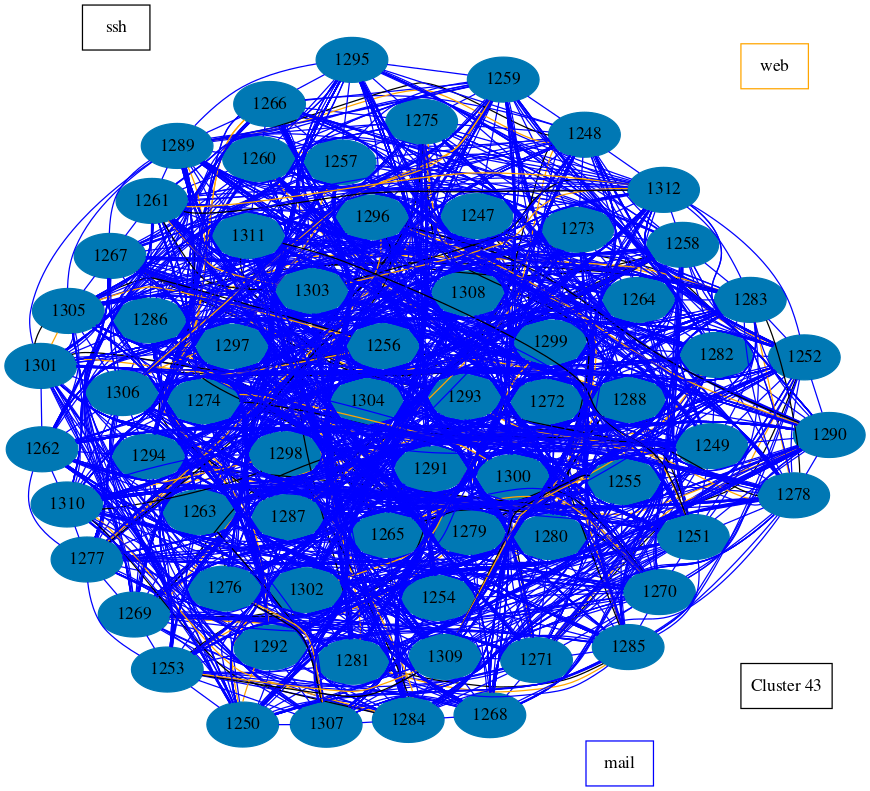
\includegraphics[width=14cm]{graph43.png}
    \caption{Cluster 43}
    \label{fig:cluster43}
\end{figure}

\noindent Figure~\ref{fig:cluster43} represents Cluster 43 from the results. It is a cluster consisting of 66 hosts sharing the same keys for SMTP, SSH and HTTPS protocols. 
All of the hosts belong to the same Autonomous System in this case. There are about 722 host-port combinations, with 86 of them being SSH. There were only 14 unique SSH keys seen for the 86 host-port combinations. Out of the 722 host-port combinations, 636 
were TLS ports with only 22 unique TLS keys seen. The AS in question here is a web-hosting service with a local presence. 
\pagebreak

\subsection{Cluster 72}
\begin{figure}[h!]
    \centering
    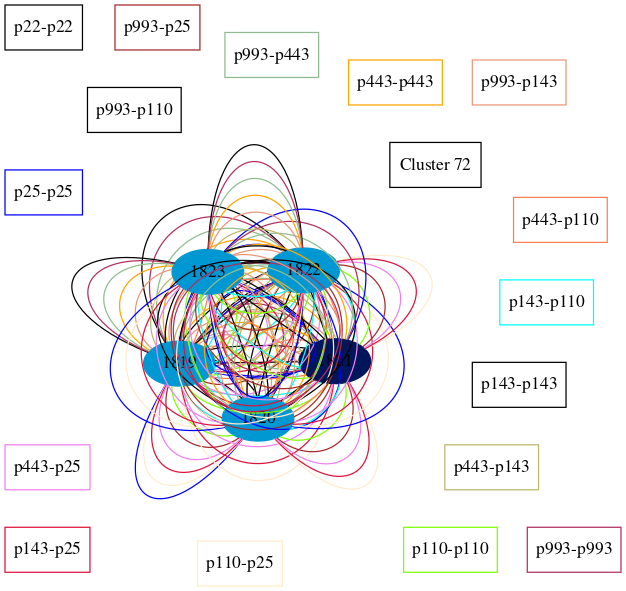
\includegraphics[width=14cm]{graph72.png}
    \caption{Cluster 72}
    \label{fig:cluster72}
\end{figure}

\noindent Figure~\ref{fig:cluster72} is an interesting one. Key sharing across almost every pair port combination is observed. There are five hosts in this cluster, 
out of which four belong to the same AS. There is key sharing across all mail protocols, but even cross-protocol key sharing among hosts for HTTPS and SMTP, IMAP and POP3 is observed. 
Upon inspection of the cluster data, it was found that the four ASes that are the same are again a web-hosting service, while the other AS seems to belong to a Telecommunications company.  
\pagebreak

\subsection{Cluster 133}
\begin{figure}[h!]
    \centering
    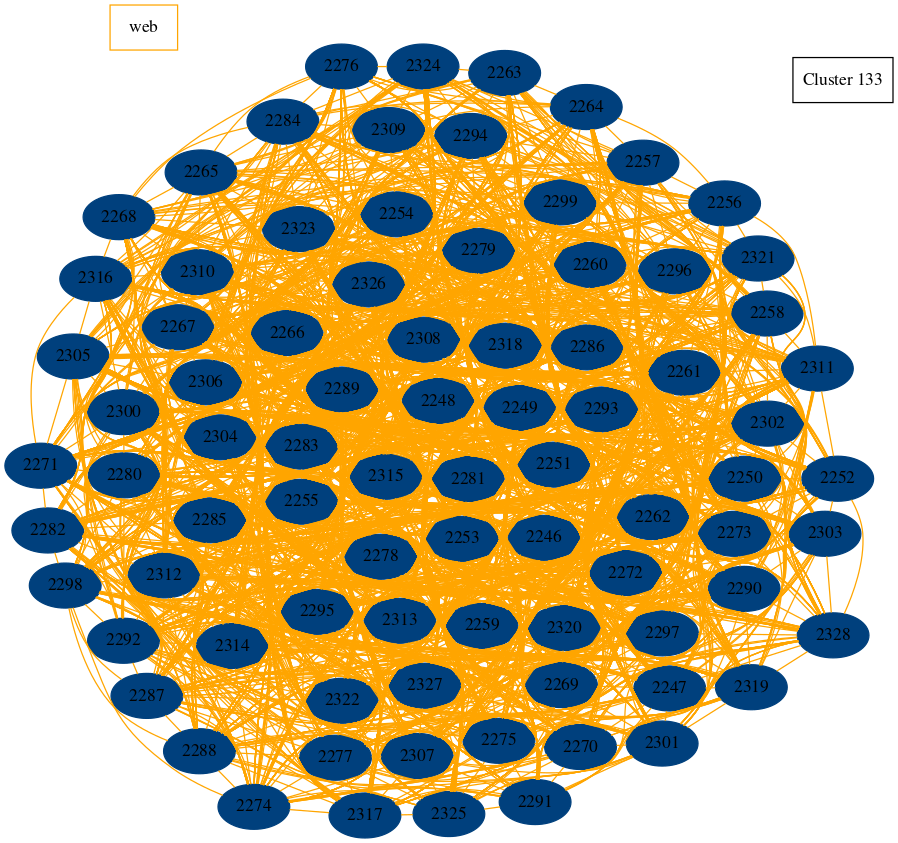
\includegraphics[width=14cm]{graph133.png}
    \caption{Cluster 133}
    \label{fig:cluster133}
\end{figure}

\noindent Figure \ref*{fig:cluster133} represents Cluster 133 from the results, and it consists of 83 hosts sharing web server keys (HTTPS). This is one of the busier clusters found in the results, and there are a few clusters 
larger than this. All 83 hosts belong to the same AS, a global web hosting service, and share keys for only port 443. There are about 166 host-port combinations, sharing only a single TLS key. 
\pagebreak

\subsection{Cluster 148}
\begin{figure}[h!]
    \centering
    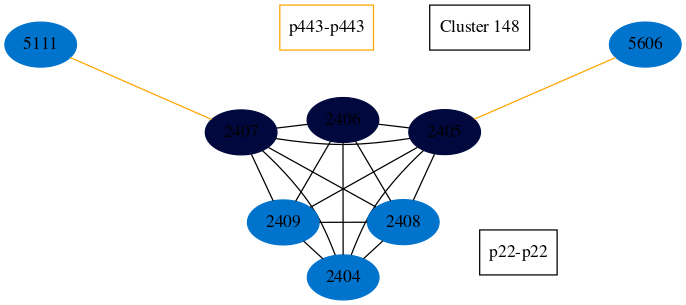
\includegraphics[width=16cm]{graph148.png}
    \caption{Cluster 148}
    \label{fig:cluster148}
\end{figure}

\noindent Figure \ref{fig:cluster148} represents Cluster 148 and consists of eight hosts belonging to two different ASes. Out of the eight, three belong to the same AS and 5 to a different one.  
All hosts in the middle share keys for SSH, while the the two host \textit{5111} and \textit{5606} (refer figure) at the edges share keys 
with the hosts \textit{2607} and \textit{2605} for port 433 respectively. There are about 22 host-port combinations seen,
out of which 12 are classified as SSH, and the remaining 10 are TLS. Only 1 SSH key is shared among the 12 host-port combinations, while 3 TLS keys are shared for ten host-port combinations. The AS with three hosts belong to a local ISP, and the other one with five hosts 
belongs to a telecommunications entity with a huge local presence. 
\pagebreak

\subsection{Cluster 536}
\begin{figure}[h!]
    \centering
    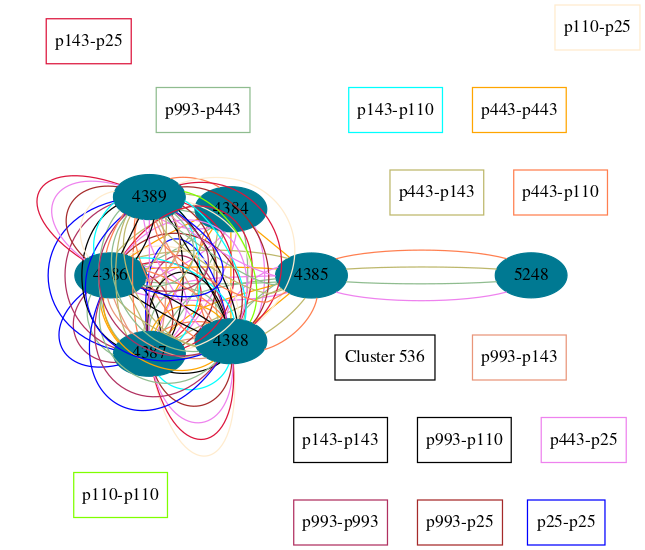
\includegraphics[width=16cm]{graph536.png}
    \caption{Graph 536}
    \label{fig:cluster536}
\end{figure}
\noindent Figure~\ref{fig:cluster536} represents Cluster 536 and has about seven hosts, all belonging to the same AS. There are seven hosts with 58 
hosts-port combinations and only four unique TLS keys. Key reuse across almost port combinations is seen here. The max key usage for a single seen 
was 38 times in this cluster. The hosts involved in this cluster seem to provide web services like mail and DNS using cloud platforms.
\pagebreak

\subsection{Cluster 786}
\begin{figure}[h!]
    \centering
    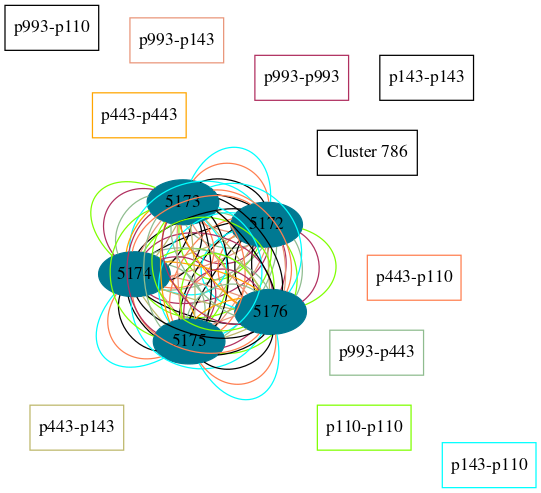
\includegraphics[width=12cm]{graph786.dot.png}
    \caption{Cluster 786}
    \label{fig:cluster786}
\end{figure}
\noindent Figure~\ref*{fig:cluster786} consists of five hosts; all belong to the same AS and share keys for TLS. There were 40 host-port combinations 
with only two TLS keys, out of which one of the keys was reused 38 times. This cluster is interesting as one of the hosts has a domain name that belongs to 
Trinity College, Dublin. The domain name associated was on port 443 (HTTPS). For instance, if Trinity's website is ``www.tcd.ie'', the 
domain name in question here looked like ``www.tcdxxxx.ie''. The AS here is a telecommunications company in Ireland. 
\pagebreak

\subsection{TLS Cipher Suites}
The TLS Cipher Suites seen for the selected clusters:
\begin{figure}[h!]
    \centering
    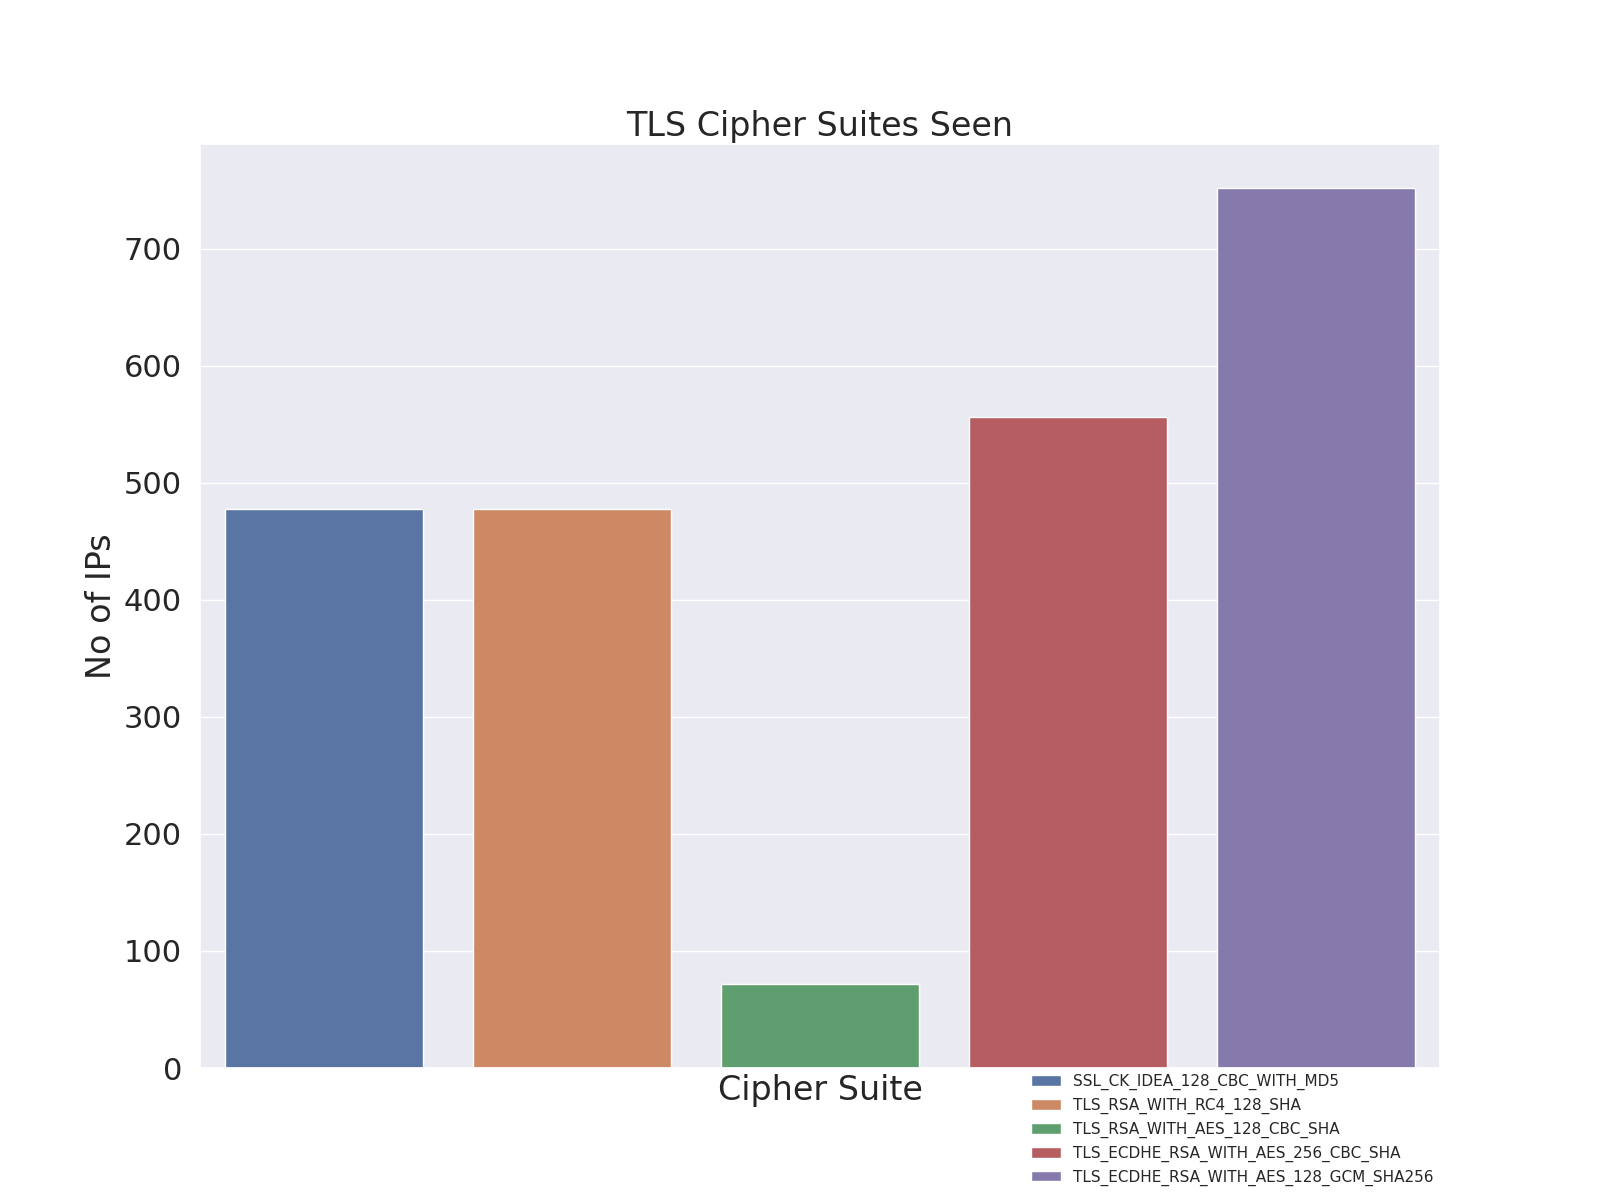
\includegraphics[width=17cm]{newgraph.png}
    \caption{TLS Cipher Suites}
    \label{fig:tlsciphers}
\end{figure}

\noindent Table~\ref*{fig:tlsciphers} shows the TLS cipher suites seen for the selected clusters. The most common cipher suite was found to be \verb|TLS_ECDHE_RSA_WITH_AES_128_GCM_SHA256| followed by 
\verb|TLS_ECDHE_RSA_WITH_AES_256_CBC_SHA|. Many hosts were using \verb|TLS_RSA_WITH_RC4_128_SHA|, which is known to have cryptographic weaknesses. The IETF prohibits the 
use of any RC4-based Cipher Suite as they do not provide desired security~\cite{rfc7465}. The least used Cipher Suite was \verb|TLS_RSA_WITH_AES_128_CBC_SHA|.
There were also significant hosts using the \verb|SSL_CK_IDEA_128_CBC_WITH_MD5| cipher that was introduced in 1992. Since then extensive studies have 
been carried out on it and is known to be broken.~\cite{rfc6151}
\newpage

\section{Post Refactoring and Optimisation}
This section discusses the results obtained after code refactoring. The profiling is done again after 
making the changes and modifications in the program. There is also a timing graph presented 
that compares the average time per IP spent analysing using the two DNS setups.
\begin{figure}[!h]
    \centering
    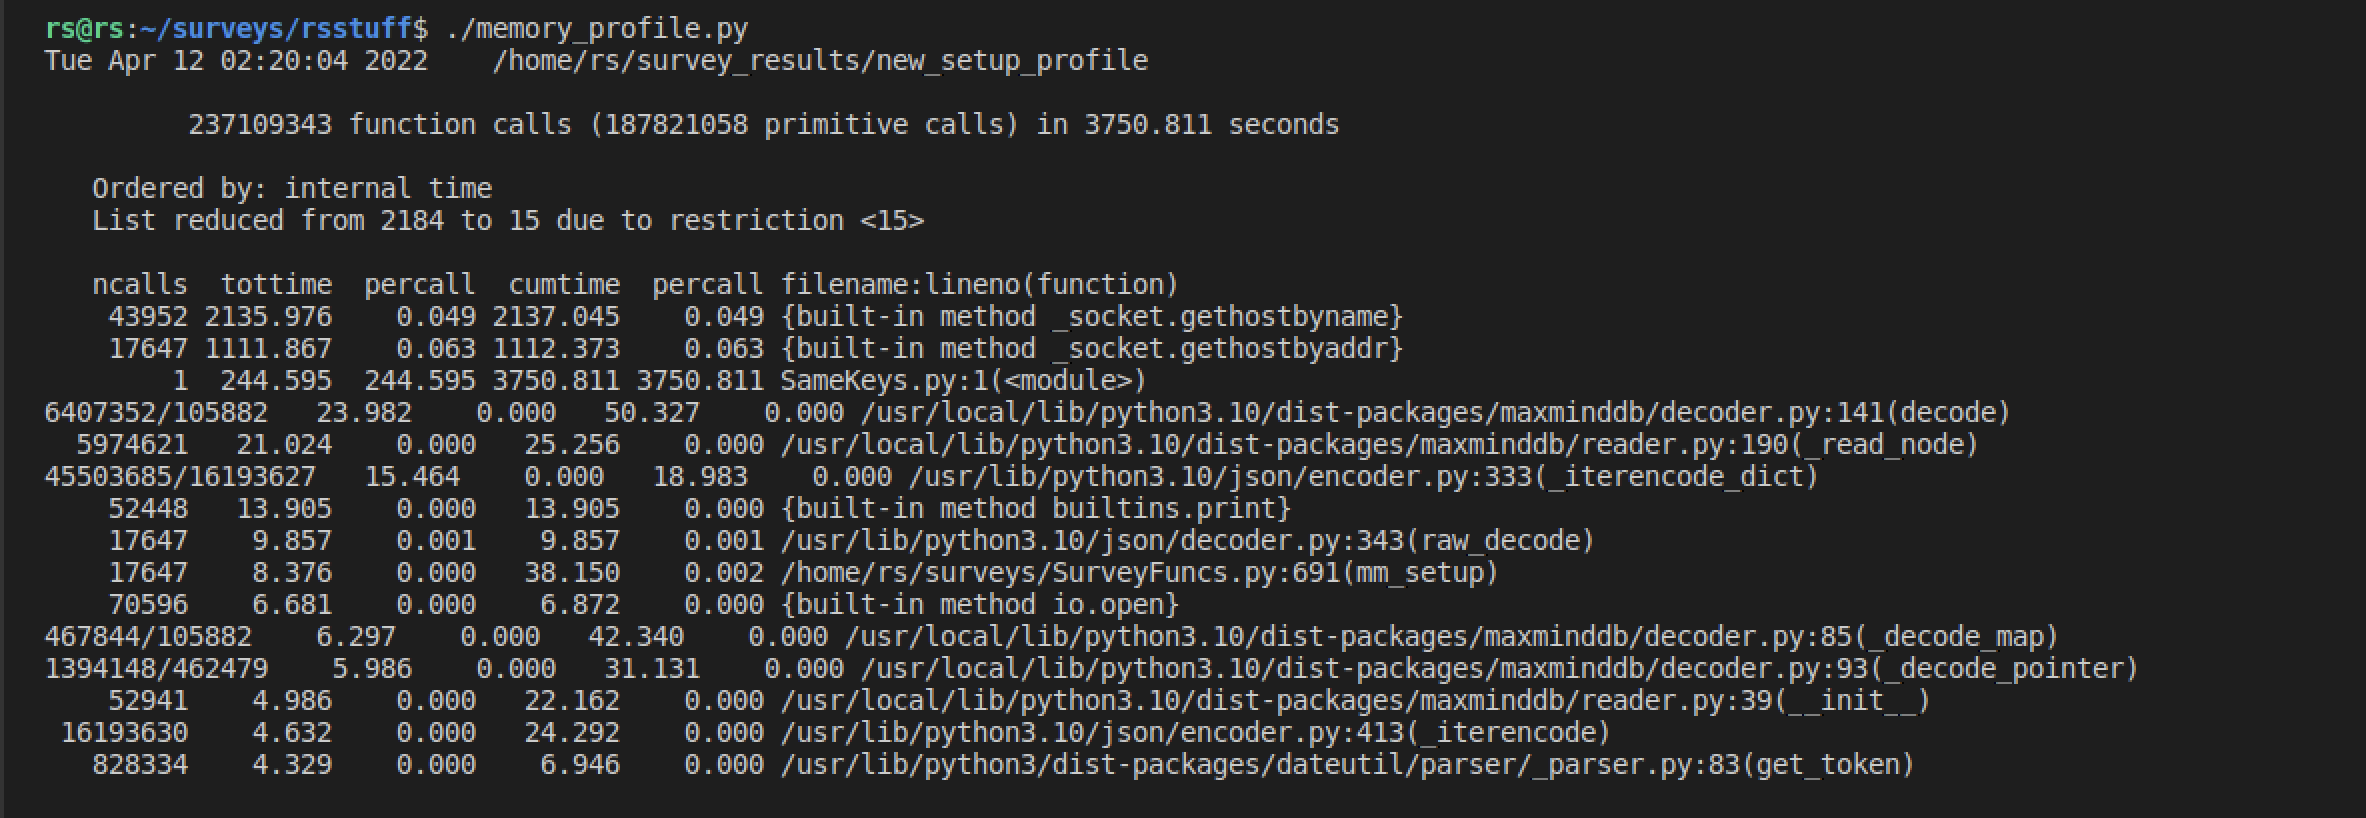
\includegraphics[width=17cm]{new_mem_profile.png}
    \caption{Memory Profile after Refactoring}
    \label{fig:memprofileafter}
\end{figure}

\noindent Figure~\ref*{fig:memprofileafter} represents the memory profiling after refactoring and optimisation as depicted in the sections above. 
The runtime for data processing and analysis was reduced from 73816 seconds to 3750 seconds. In addition, after refactoring, the number of recursive calls 
were reduced, contributing to optimising the memory consumption as recursive methods can take up a lot of memory. The new DNS setup 
significantly improved the runtime of the program, and this might be due to the following factors:
\begin{itemize}
    \item Typical DNS setups rely on servers supplied by ISPs that might be slow. 
    \item Configurations for caching might not be adequately implemented by the ISP, which may contribute to slow lookups.~\cite{HowandWh90:online}
\end{itemize}
\pagebreak

\begin{figure}[h!]
    \centering
    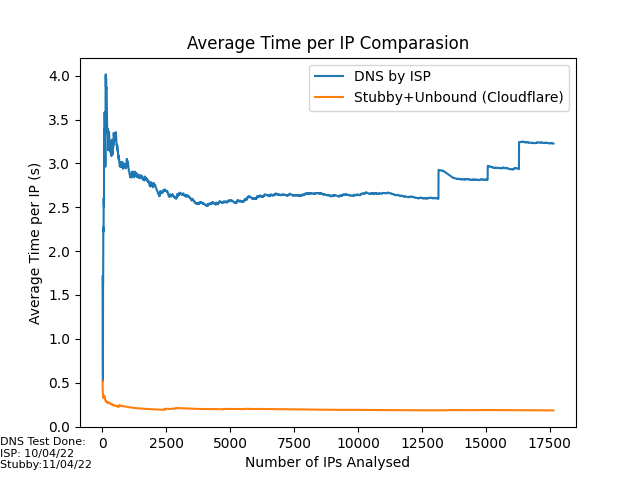
\includegraphics[width=15cm]{newdnscomp.png}
    \caption{DNS Setup Comparisons}
    \label{fig:dnscomps}
\end{figure}

\noindent Figure~\ref*{fig:dnscomps} above shows the difference between the average time spent per IP when using the two DNS setups.
The average time processing each IP was bought down to 0.15s from 3.4s when using the default setup. This might be due to the following 
reasons:

\begin{itemize}
    \item Using Unbound, one can get more control over their DNS setup as it allows one to configure the DNS servers one might want to use. 
    \item It will also cache all queries made for faster lookups the next time. 
    \item Using Stubby allows one to use DNS over TLS for sending queries to resolvers. It allows for increased privacy. 
    \item Since Unbound is not as advanced as Stubby and does not have the provision to use the same TLS connection for queries, a combination
    of the two can help speed things up. Stubby can use the same TLS connection to make multiple queries, saving the overhead and time to open up 
    a new connection for each query.~\cite{NLnetLab67:online, DNSPriva7:online}
\end{itemize}
